\subsection{The Language of the System}
\label{LanguageOfTheSystem}

Rich Hickey is most widely known as the creater and
\textit{Benevolent Dictator for Life} (BDFL) \cite{bdfl} of
\textit{Clojure} \cite{clojure2008}, \cite{clojure2010},
\cite{clojure.org}, \cite{clojure-rationale},
a functional programming language and Lisp \cite{lisp86},
\cite{commonlisp90} dialect.
Clojure runs on the Java virtual machine to allow Java and Clojure interop
in order to utilize the extensive collection of already existing
Java libraries.

Clojure is therefor not a \textit{pure} \cite{pure}
functional programming language but should rather be considered a
pragmatist's compromise of having immutable data by default but
allowing for easy I/O and statefulness whenever neededed.

Although Clojure's \textit{front end} (its syntax) looks a lot like
Lisps syntax, which is notorious for its extensive use of
parenthesis, Clojure's \textit{back end} (its implementation)
focusses heavily on very modern features like
\textit{software transactional memory} \cite{stm} and
\textit{persistent data structures} \cite{persistentdatastructures}
aimed at highly concurrent programming.

Hickey himself has been promoting these features as necessary
upgrades to the object oriented view on programming in order to
fully utilize multicore architectures and is an avid
visitor of conferences of programming language design. He therefor has
a considerable collection of talks and lectures in which he explains
his rationale behind his design decisions \cite{hickey-talks},
\cite{hickey-bestof}.
\newline

One of his more relevant talks regarding the work presented here
is called ``The Language of the System''
\footnote{In the context of this talk and for the rest of the work presented
here the word \textit{system} does not mean \textit{low-level} or
\textit{bits and bytes} as in operating system but rather means
the system as a whole as from a bird's-eye view and more as
described by something like systems theory.}
held at \textit{Clojure Con} 2012 \cite{hickey-systemlang},
\cite{clojurecon}.
In it Hickey criticizes what has already been outlined in
chapter \ref{actorModel}, namely that distributed \textit{systems}
today are being built indirectly by programming individual units and
components and then running them simultaneously, hoping that a
distributed system will almost magically emerge but lacking any
description whatsoever of that system as a whole.

\begin{wrapfigure}{r}{0.5\textwidth}

  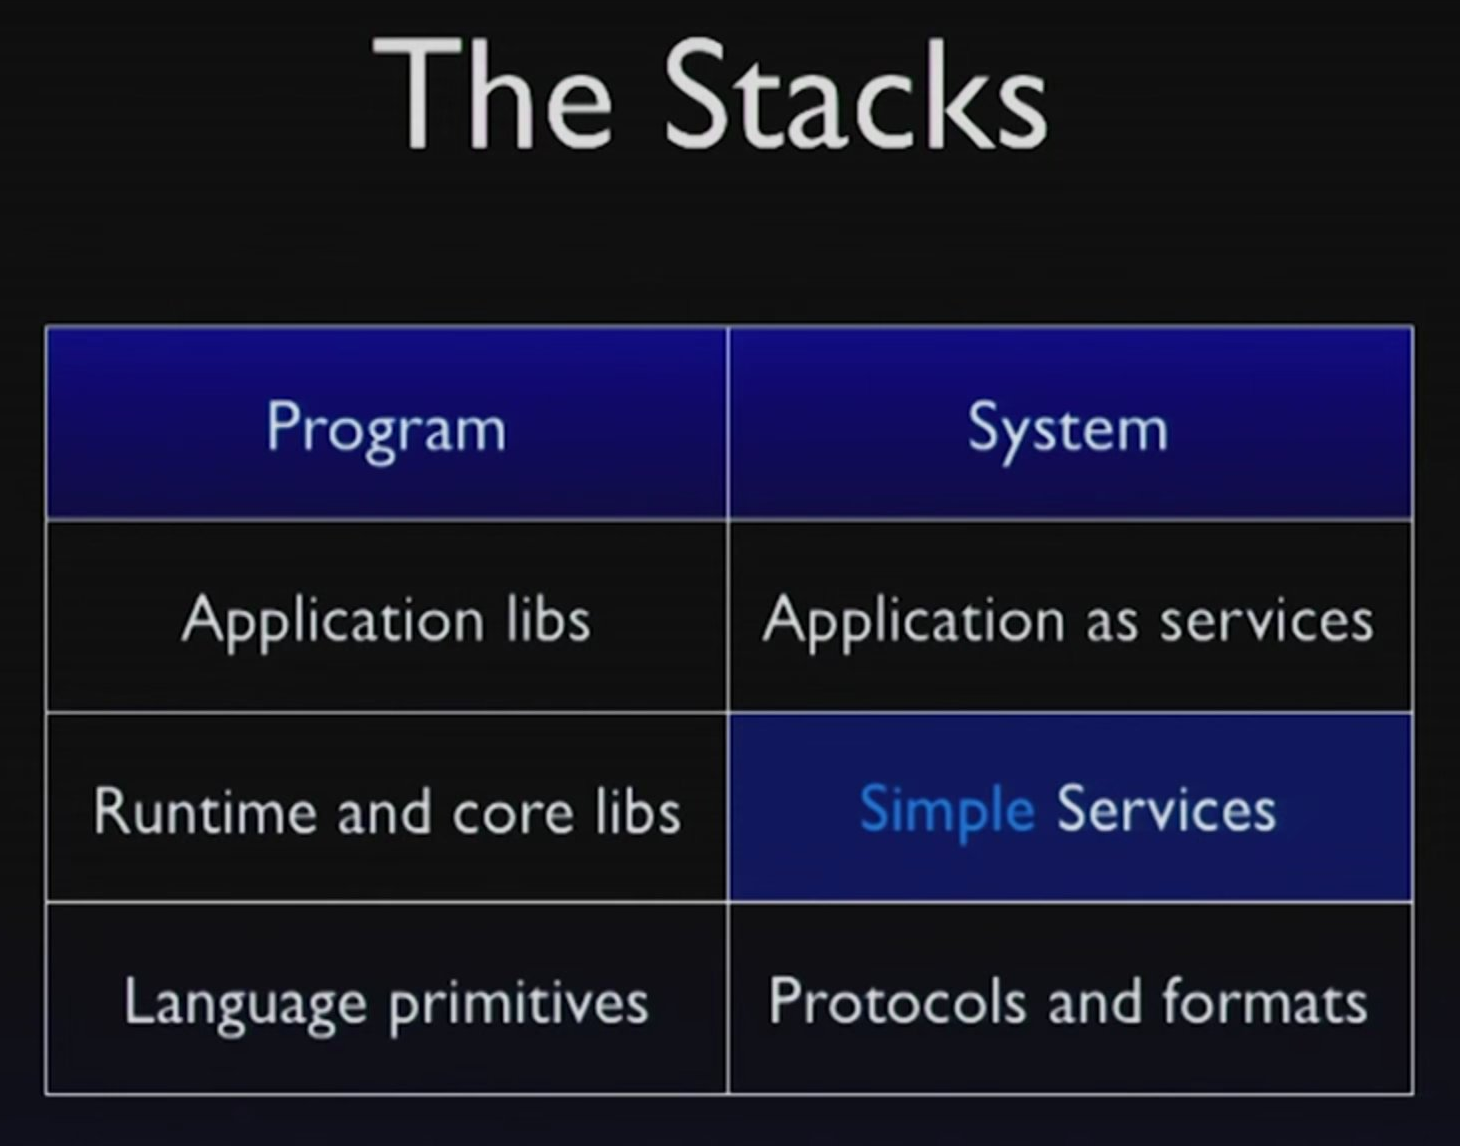
\includegraphics[width=0.5\textwidth]{systemlang.png}
  \caption{Slide-excerp from the talk ``The Language of the System'' by
          Rich Hickey that draws parallels between the composition of
          (local) programs and distributed systems.}
  \label{systemlang}

\end{wrapfigure}

The reason for this, he claims, is that the languages and tools
we use to build each individual component have been developed to
do exactly this: describe \textit{programs}, describe encapsulated
self-contained blocks of computation. They don't provide any
means of describing how to compose these components, because they
don't provide any primitives for how they \textit{communicate}.

As can be seen in Fig.\ref{systemlang} he draws parallels to how
we haven been building our programs in order to derive similar
properties for our system composition and description. For example
he proposes that the language of the system too, would have
primitives just like the programming languages that we have been
using so far. But instead of having primitives of computation like
built-in data types and arithmetic operators, in the systems context
these primitives would be primitives of \textit{communication} like
communication protocols or data formats. On top of which simple
core services need to be available in order to compose higher
level application logic, just like core libraries like
the GNU C library (glibc) \cite{glibc} or any other standard
library of any common programming language provide essential
building blocks for programmers to compose their programs.
\newline

So the relevance of this talk to the work presented here is, that
it sparked the question of whether or not it would be possible to
build such a composition language of the system that allowed a
global perspective without introducing global state and how such a
language would look like.
\newline

The other talk by Hickey which is relevant to this work and which
I would like to summarize here is called ``The value of values''
and was held at the GOTO Conference 2012 as well as the JaxConf 2012
\cite{vofv-infoq}, \cite{vofv-yt}, \cite{goto2012}, \cite{jax2012}.
Probably being his most famous talk, in it Hickey bootstraps his
views on programming and language design by putting
\textit{immutable data} at the center of programming and deriving
the advantages of core functional programming concepts from that.
He introduces two programming paradigms,
namely \textit{place-oriented programming} and
\textit{value-oriented programming}. A \textit{place} in Hickey's
view literally represents a place in reality. Something where
one can put things and where they reside. If one replaces the thing
that already resides in a place with some other thing, the
information of that exchange is never recorded. Places don't
record their exchange \textit{history} so to speak. Every exchange
\textit{overwrites} the current content of that place.
To the effect that the value received from querying a place
depends on the point in \textit{time} when the query was executed.
The value of the place is inherently intertwined with time, which
is what is generally known as \textit{state}.

This represent the bulk of programming language history. It
even represents the slots on the band of a Turing machine, which
can be overwritten by said Turing machine with symbols defined in
its alphabet. We have built hardware like memory and hard drives
but also our software like data bases and file systems
after this principle. They provide slots of storage which can
carry a value but can be overwritten so the new value replaces the
old and the value received from querying a place depends on the
moment in time of the query.

\begin{wrapfigure}{r}{0.6\textwidth}

  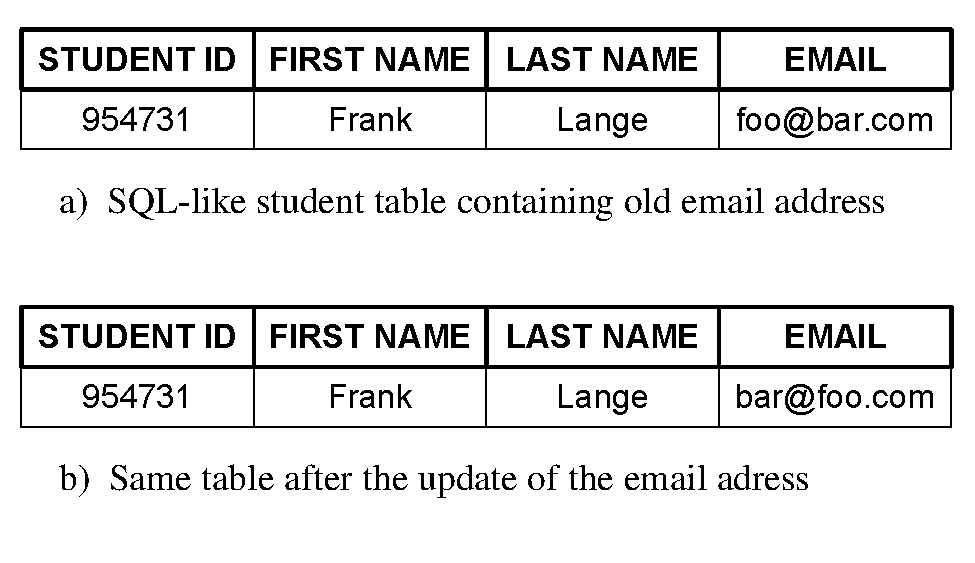
\includegraphics[scale=0.6, keepaspectratio]{sql.pdf}
  \caption{Place-orientation examplified by a SQL table, each cell
           being a place.}
  \label{sql}

\end{wrapfigure}

In order to examplify this concept, Fig.\ref{sql} shows a very
basic representation of what could be a \textit{SQL} table.
This table stores data using the schema of \textit{(ID, First Name,
Last Name, Email)} which is supposed to represent a registered
student. In Hickey's view, each cell of the table is a place, so
if a student were to change her email address only the cell containing
the email address would change, as shown in Fig.\ref{sql}b.
But changing an email address does not invalidate the fact that
there has been a point in time in which the student used the
old email address, just like electing a new president of a country
does not




